\documentclass{article}
\usepackage{graphicx}
\usepackage{amsmath}
\usepackage{fixltx2e}
\usepackage{float}


\begin{document}

\title{Software package for Engineering drawing}
\author{Aditya Jain \& Ankit Akash}

\maketitle

\begin{abstract}
Drawing is precisely considered as a Universal Language. For ages the depiction of a 3D object in 2D sheets has been a problem of sheer importance. People have relied on orthographic methods of projection to ensure unambiguous communication for proper convey of graphic ideas. This method although being simple requires a level of imagination on both the parties to properly visualize the 3D body from 2D views. The motive here is to automate the process of projection from 3D to orthographic views and reconstruction from the same.
\end{abstract}



%%%%%%%  1st Part  %%%%%%%%


\part{3D object to Orthographic Projections}

\section*{Idea}
For projection of a 3D object onto any 2D plane we assume that the object has no line attribute ,it has only collections of points which represent the whole object. This helps in generalizing the concept of projections for curves and transformation of the object.

\section{Transformations on 3D Object}
The coordinate points \((x,y,z)\) can be transformed using the five basic operations which are translation,rotation,reflection,scaling and shearing. These operations will help us in getting the different views of the object by converting the coordinates into the new transformed ones. 
We use the row vector \((x,y,z,1)\) to get the transformed coordinates by multiplying it with the transformation matrix.

\subsection{Translation}
To shift a point by \((t\textsubscript{x},t\textsubscript{y},t\textsubscript{z})\) we multiply its \(4\) dimensional row vector by the translation matrix which is given below and denoted by T.


\begin{equation}
    \label{simple_equation}
    T(t_x,t_y,t_z) = \begin{bmatrix}1 & 0 & 0 & 0 \\0 & 1 & 0 & 0 \\0 & 0 & 1 & 0 \\t_{x} & t_{y} & t _{z} & 1 \end{bmatrix}
\end{equation}

\subsection{Scaling and Reflection}
Scaling the object about the origin by a factor of s\textsubscript{x},s\textsubscript{y},s\textsubscript{z} in x,y and z directions respectively is done by multiplying with the following scaling matrix
\begin{equation}
    \label{simple_equation_2}
    S(s_x,s_y,s_z) = \begin{bmatrix}s_{x} & 0 & 0 & 0 \\0 & s_{y} & 0 & 0 \\0 & 0 & s_z & 0 \\0 & 0 & 0 & 1 \end{bmatrix}
\end{equation}
The transformation matrices of the reflection R\textsubscript{yz} in x=0 plane , R\textsubscript{xz} in the y=0 plane, and R\textsubscript{xy} in the z=0 plane are obtained by scaling of -1 in the respective axis .
\begin{equation}
    \label{simple_equation_3}
    R_{yz} = \begin{bmatrix}-1 & 0 & 0 & 0 \\0 & 1 & 0 & 0 \\0 & 0 & 1 & 0 \\0 & 0 & 0 & 1 \end{bmatrix}
    \end{equation}
    \begin{equation}
    \label{simple_equation_4}
    R_{xz} = \begin{bmatrix}1 & 0 & 0 & 0 \\0 & -1 & 0 & 0 \\0 & 0 & 1 & 0 \\0 & 0 & 0 & 1 \end{bmatrix}
    \end{equation}
    \begin{equation}
    \label{simple_equation_5}
    R_{xy} = \begin{bmatrix}1 & 0 & 0 & 0 \\0 & 1 & 0 & 0 \\0 & 0 & -1 & 0 \\0 & 0 & 0 & 1 \end{bmatrix}
\end{equation}

\subsection{Rotations About the Coordinate axis}
The transformation matrices for rotation about the x,y and z axis are Rot\textsubscript{x},Rot\textsubscript{y} and Rot\textsubscript{z} respectively given by:
\begin{equation}
    \label{simple_equation_6}
    Rot_{x}(\theta_{x}) =\begin{bmatrix}1 & 0 & 0 & 0 \\0 & \cos\theta_{x} & \sin\theta_{x} & 0 \\0 & -\sin\theta_{x} & \cos\theta_{x} & 0 \\0 & 0 & 0 & 1 \end{bmatrix}
\end{equation}
\begin{equation}
    \label{simple_equation_7}
    Rot_{y}(\theta_{y}) =\begin{bmatrix}\cos\theta_{y} & 0 & -\sin\theta_{y} & 0 \\0 & 1 & 0 & 0 \\\sin\theta_{y} & 0 & \cos\theta_{y} & 0 \\0 & 0 & 0 & 1 \end{bmatrix}
\end{equation}
\begin{equation}
    \label{simple_equation_8}
    Rot_{z}(\theta_{z}) =\begin{bmatrix}\cos\theta_{z} & \sin\theta_{z} & 0 & 0 \\-\sin\theta_{z} & \cos\theta_{z} & 0 & 0 \\0 & 0 & 1 & 0 \\0 & 0 & 0 & 1 \end{bmatrix}
\end{equation}

\begin{figure}[h]
  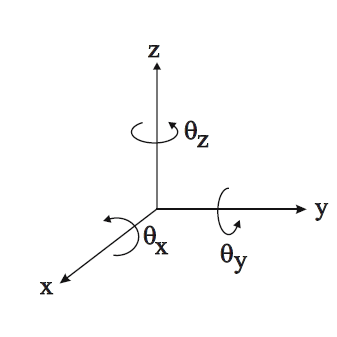
\includegraphics[width=10cm,height=10cm]{axis.png}
  \caption{Positive angles of rotation}
  \label{fig:boat1}
\end{figure}

\subsection{Rotation About An Arbitrary Line In Space}
Rotation through an angle $\theta$ about an arbitrary rotation axis is obtained by transforming the rotation axis to one of the coordinate axis , applying a primary rotation through an angle $\theta$ about the coordinate axis and then tracing back to the rotation axis. 
\\Let the rotation axis have cosines $(c_1,c_2,c_3)$. If the rotation axis passes through point P $(p_1,p_2,p_3)$ then applying the following transformation matrices will rotate the coordinates :
\\ (1) Apply the translation $ T(-p_{1},-p_{2},-p_{3})$ which maps the point P to origin.
\\ (2)Apply a rotation through an angle $\theta_{x}$ about the x-axis so that the line is mapped into the $xz$-plane.
\\ (3)Apply a rotation about the y-axis so that the line is mapped to the $z$-axis .
\\ (4)Apply a rotation through an angle $\theta$ about the $z$-axis.
\\ (5)Apply the inverses of the transformation 1-3 in reverse order.

$$    T(-p_{1},-p_{2},-p_{3})Rot_{x}(\theta_{x})Rot_{y}(-\theta_{y})Rot_{z}(\theta)Rot_{y}(\theta_{y})Rot_{x}(-\theta_{x})T(p_{1},p_{2},p_{3})$$
where 
$$\sin\theta_{x} = \frac{c_2}{\sqrt{c_2^2+c_3^2}}  \cos\theta_{x} = \frac{c_3}{\sqrt{c_2^2+c_3^2}} $$
$$ \sin\theta_{y} = c_1 , \cos\theta_{y} =\sqrt{c_2^2 + c_3^3}$$
\section{Projection From 3D to 2D Generalizations }
Each edge is divided into numerous points hence we end up have cloud of points. Points are named uniquely. We project each point on the surface. Then we tag to each projected point a label h or p with the corresponding meaning :-
\begin{itemize}
\item H - The point is a part of a edge that is hidden
\item S - The point is a part of a edge that is solid in that view
\end{itemize}

\section{Projection on arbitrary cross section}
Lets say we have a plane \ ax + by + cz + d = 0\
We want projection of a random point \ (x,y,z)\
We do the following math :-
 \[ t = \frac{ax_1+by_1+cz_1+d}{a^2+b^2+c^2} \]
 \[ (x_p,y_p,z_p)=(x_1,y_1,z_1)\times(1-t) \]
\((x_p , y_p , z_p)\) represent projection of a single sample point. 
The collection of all \((x_p , y_p , z_p)\) forms its 2d projected figure.



\begin{flushleft}
%%%%%%%  Needs editing, down  %%%%%%%%
\\If the normal to the plane is given then we can also rotate the whole object such that the z-axis of the newly rotated object aligns with the given normal . Then we can take the orthographic projections as before.
\\To align the z-axis with the normal let the unit vector of normal be denoted by $u$. Then by using Rodrigue's rotation formula :
$$v_{rot} = v\cos\theta + (k \times v )\sin\theta + k(k.v)(1-\cos\theta)$$
where $$k=\frac{u\times\hat{z}}{|u\times\hat{z}|} $$
$v_{rot}$ is the final rotated vector and $v$ is the initial vector.So by applying this formula to all the vertices we can align our object to the given normal .
\end{flushleft}
\section{Projection on standard xy, yz and zx planes}
Drop the corresponding coordinate x or y or z like wise:-
\begin{itemize}
\item For xy plane - drop z
\item For yz plane - drop x
\item For xz plane - drop y
\end{itemize}
Add the label.

\section{How to label H and S}
Theoratical Idea : We extend our 3d object to form a mesh of points enclosing the whole surface of our object. For marking solid and dashed lines in any view (say, xy) we proceed by projecting parallel lines in the direction of normal vector (in this case z-axis) from each projected point. The point at which this line meets our 3d object for the first time is the one which will be visible when viewed from the surface. Rest all points lieing in that line would be hidden from our sight with respect to that view. Thus we get a simple scheme, mark point S if it's first intersection, H otherwise. 
Once the labelling is done, join all the S points with dark lines, H points with dashed lines.

%%%%%%%  2nd Part  %%%%%%%%

\part{Converting Orthographic Projections}
\setcounter{section}{0}
\section{How to store them?}
A 2D orthographic figure is a collection of tuples we name as 2dVertices, Edge1 and Edge2.2dVertices(V) represents intersection of edges. It is collection of points with pair of integers x,y denoting respective position in the axis. Any edge e in Edge1 or Edge2 is of the type v1xv2 where v1,v2 E V. Hence Edge1 and Edge2 are subsets of VxV. Each edge e1 in Edge1 represent a solid line in the isometric view. Each edge e2 in Edge2 represent a dashed (hidden) line in the isometric view. For a single object we have 3 sets of {V, Edge1 and Edge2} with labels as Top, Front and Side.
\section{How a object data looks for 3D?}
3D space consists of 3dVertices, Edges, Planes.
3dVertices are basic building blocks. It is collection of tuples with 3 integers x,y,z representing vertex’s position in 3D space.
Similar as previous definition any edge e in Edges is of the type v1xv2 where v1,v2 E V. Hence Edge1 and Edge2 are subsets of VxV. Each edge e1 in Edges represent a line between its corresponding vertices in 3d view.
Planes is a tuple of arbitrary size containing a collection of 3dVertices where each of the Vertices lie in the literal same plane

\section{How to transfer information from 2D projections to get 3D object?}
We have 
\begin{table}[h!]
\centering
\begin{tabular}{||c c c c||} 
 \hline
 Front View(X-Z) & Front View(X-Z) & Front View \\ [0.5ex] 
 \hline\hline
 V1(x,z) & V1(x,z) & V1(x,z) \\ 
 Edge11 & Edge11 & Edge11 \\
 Edge21 & Edge21 & Edge21 \\ [1ex] 
 \hline
\end{tabular}
\label{table:1}
\end{table}
Every vertex in 3D space is uniquely defined by triplet x,y,z. We propose a simple Algorithm to construct the 3dVertices list for 3D representation :-
\begin{itemize}
\item Construct a blank list Vertices’’ of type 3dVertices
\item For all v1 in V1
\item For all v in Vertices’’ extract y,z to get a a a 2dVertex in 2dVertices.
\item Vertices’ contains all the corresponding points that the object will have which we would obtain by the given 2d projections.

\end{itemize}


\section{Problem with our Algorithm}
It evaluates and gives all the points that our object should have(Why?: proof is obvious) but it also reports extra points that doesn’t belong to the object(say shadow points). Consider this as example :-

\begin{figure}[H]
  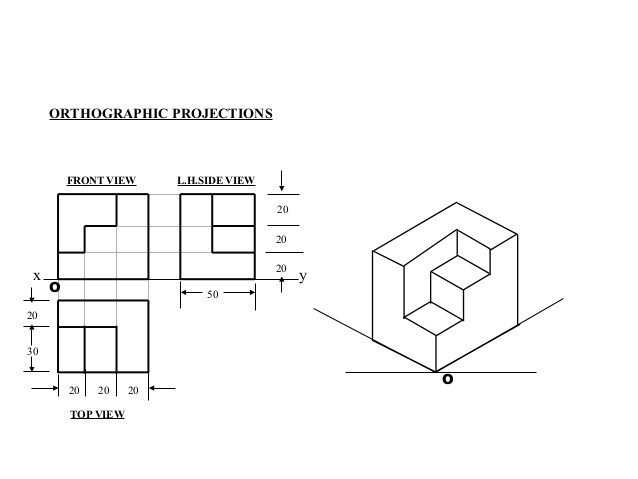
\includegraphics[width=15cm,height=10cm]{unit-6-isometric-views-28-638.png}
  \caption{Example}
  \label{fig:boa}
\end{figure}

Applying the algorithm gives a shadow point in extra i.e. the deleted edge of the original cube.
And this thing in general happens with all those points which can be formed in our 3d object by extending any three line segments in 3d object till infinity(ofcourse, its possible only if the 3 are concurrent).  So how can we handle this? By the basic fact that

\section{Edges too in isometric drawing carry information}
This simple fact has not been utilised until now. But it too carry a powerful piece of information for reconstruction of our 3d object. If two edge in our drawing are collinear and concurrent at one point then the other points forming the edge must have different z component (note here z is arbitrary reference to the third unknown component of the 2dVertex). 
Addition of this small fact enables our algorithm to eliminate the shadow points. 
Now lets restrict ourselves to simpler case when each vertex in 2dVerteices carry a label which shows which 3d object it belongs to.
\section{Original Problem Statement}
Using information from set of isometric projections of a 3d object to reconstruct it back identically. Here each of the 2d figure in isometric projection carry information of 
\begin{itemize}
\item Vertex position(x,y) with label
\item Edge list for solid lines and 
\item Edge list for hidden lines. 
\end{itemize}
\section{Converting Wireframe To Solid Structure}
There are two models for converting a wireframe into a solid structure. One is volumetric model and the other is surface model. We will be sticking with the latter one in this program. For the surface model we need to find all the faces which are produced by closed edge loops .First we will produce all the faces which are possible then remove the pseudo-faces by using a set of rules which are defined below . Finally all the true faces are assembled to form the solid object. 
\subsection{Finding All The Possible Faces}
As our object is polyhedral all its faces will be planar and so to find the faces we will search for closed loops formed with edges in all possible planes. A plane will be formed whenever two edges share one common vertex . Using this fact and minimum-internal-angle searching method we can find all the possible faces in the wireframe.Starting from a convex vertex (at the extreme left) we can ensure that loops have no internal edges.
\\for (each vertex, vi)
\\for (each pair of adjacent edges, $e_i$,$e_j$) do
\\n = normal to plane, $e_i$ x $e_j$
\\$v_k$ = vertex at far end of $e_j$
\\ while( $v_k$ $\neq$  $v_i$ and $e_j$ exists)
\\$e_k \longleftarrow$ edge adjacent to $v_k$, coplanar to n,with minimum-internal-angle from e,
\\$e_j$ = $e_k$; $v_k$ = far end of $e_k$
\\end while
\\if ($v_k$=$v_i$) then
\\list $ e_i,e_j,e_k,$ . . . is a possible face loop
\\end if
\\next e,,q
\\next v, 

\subsection{Rules For Detecting Pseudo Faces}
The following rules are followed while removing the pseudo faces from the set of all faces:
\\$\langle 1\rangle$When an edge is adjacent to more than two
faces, at most two faces can be true, the rest
must be pseudo. (From the Moebius rule)
\\$\mathbf{Moebius Rule:}$each edge in a manifold solid belongs to two faces and its orientation is inverted by each face.
\\$\langle 2\rangle$When two faces intersect, only one of them can
be true. (If they were both true, the intersecting
edge would have four adjacent faces contradicting Moebius rule)
\\$\langle 3 \rangle $ A dashed edge which has no face to occlude is false.(dashed line definition)
\\$\langle 4 \rangle$ If an edge is adjacent to only one face then both the face and edge are false by Moebius rule.
\\$\langle 5 \rangle$ If an edge is adjacent to two coplanar faces then the faces can be merged and the edge be removed.
\\$\langle 6 \rangle $ If a true edge is adjacent to two non-coplanar faces then both the faces are true.
\\$\langle 7 \rangle $ If a face is coplanar and adjacent to a true face and their shared edge is solid in the projected view then the the face must be false (otherwise it will contradict 5).
\subsection{Implementing Rules}
When undecided edges are found, assumptions are
made using rules 1 and 2, then rules 1 to 7 are
applied, until either all edges are decided, or no
object is found. All possible objects are detected this
way, without having to assemble them first. The
recursive algorithm is summarised as follows:
\\$\mathbf{function()}$
\\if (all edges obey Moebius rule)
and (no faces intersect) then
a solution has been found, add it to the list
\\else
\\for (each undecided edge $e_i$) do
\\for (each adjacent pair of faces$f_j ,f_k$) do
\\assume $f_i,f_k$ are true;
\\if (rules 1-7 change anything) then
\\call function
\\end if
\\next $f_j,f_k$
\\next $e_i$
\\end if
\\$\mathbf{end function}$



%%%%%%%  3rd Part  %%%%%%%%

\part{How many projections do we need?}
\setcounter{section}{0}
The three principal views are top, front and side. In engineering drawing, the choice of number of views is determined by the need to define the engineering object uniquely and unambiguously. If the corresponding labelling of points is given then two views are sufficient to describe all the corner vertices and edges of our object with certainty. What if points are labeled in correspondence  but only for those which are necessarily required to represent the 2d figure. Why are we considering this case?
Look at the figure 2 below :-

\begin{figure}[H]
  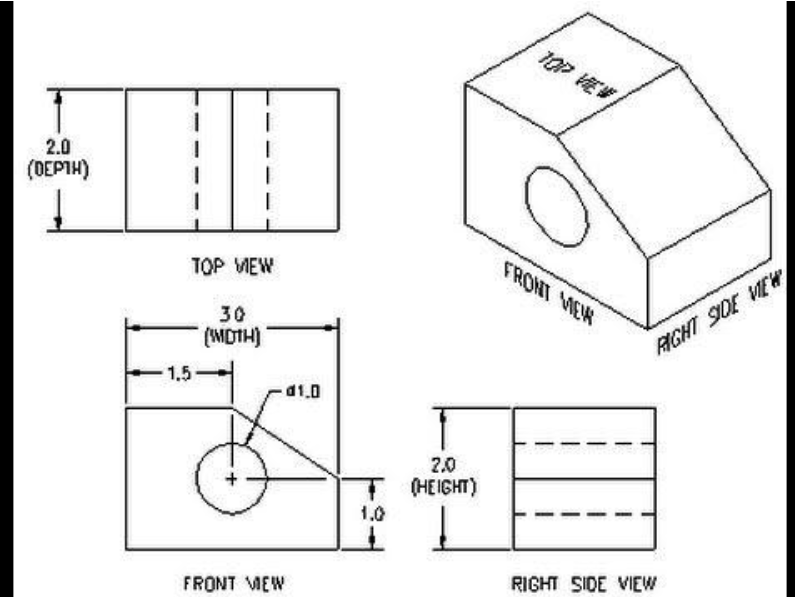
\includegraphics[width=12cm,height=8cm]{fig2.png}
  \caption{Orthographic views of an object}
  \label{fig:boat1}
\end{figure}


\\In the top and side view its ridiculous to label infinite number of points corresponding to the circular region of our object and if we approximate it by any number of finite points then there is always a confusion left out whether the hole is a polygonal cut or cylindrical. So 2 views are never sufficient to represent a 3d object reserving its identity.



\end{document}